\subsection{Flyweight (\textit{o Cache})}
\label{flyweight}

\textbf{Scopo}: Strutturale \\
\textbf{Raggio d'azione}: Oggetti

\paragraph{Definizione} Permette di supportare la condivisione di un numero grande di oggetti \textbf{fine-grained} efficientemente.

\paragraph{Motivazione} Alcune applicazioni potrebbero beneficiare dell'utilizzo di oggetti condivisi nell'intero progetto, ma un implementazione naive potrebbe risultare proibitiva in termini di costi.

La maggior parte degli editor di documenti implementa funzioni di formattazione e modifica del testo in modo modulare, utilizzando oggetti per rappresentare elementi complessi come tabelle o figure. In teoria, un approccio ancora più flessibile consisterebbe nell'associare un oggetto a ciascun carattere del documento, consentendo una gestione uniforme di caratteri ed elementi incorporati e facilitando l'estensione dell'applicazione con nuovi set di caratteri. Tuttavia, questa strategia comporta costi elevati: anche documenti di dimensioni moderate richiederebbero centinaia di migliaia di oggetti, con un consumo di memoria e un sovraccarico di runtime potenzialmente inaccettabili.

\begin{figure}[H]
    \centering
    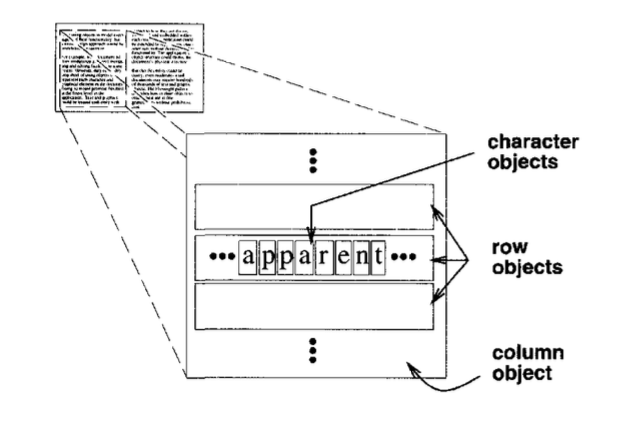
\includegraphics[width=0.5\linewidth]{assets/pattern/flyweight/flyweight-esempio.png}
\end{figure}

Il \emph{Flyweight Pattern} affronta questo problema introducendo oggetti condivisi (\emph{flyweight}) che possono essere utilizzati simultaneamente in più contesti, comportandosi come istanze indipendenti. La chiave del modello è distinguere tra \emph{stato intrinseco}, memorizzato e indipendente dal contesto (ad esempio il codice di un carattere), e \emph{stato estrinseco}, dipendente dal contesto e fornito dal client quando necessario (come posizione e stile tipografico). Questo approccio consente di rappresentare concetti molto numerosi, come i singoli caratteri di un testo, mantenendo bassi i costi di memoria e senza compromettere la flessibilità del sistema.

\begin{multicols}{2}
\begin{figure}[H]
    \centering
    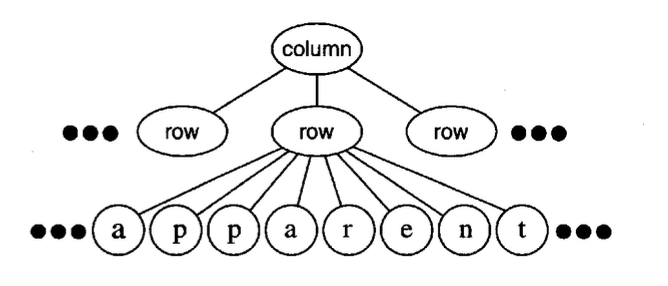
\includegraphics[width=1\linewidth]{assets/pattern/flyweight/flyweight-soluzione-1.png}
\end{figure}
\columnbreak
\begin{figure}[H]
    \centering
    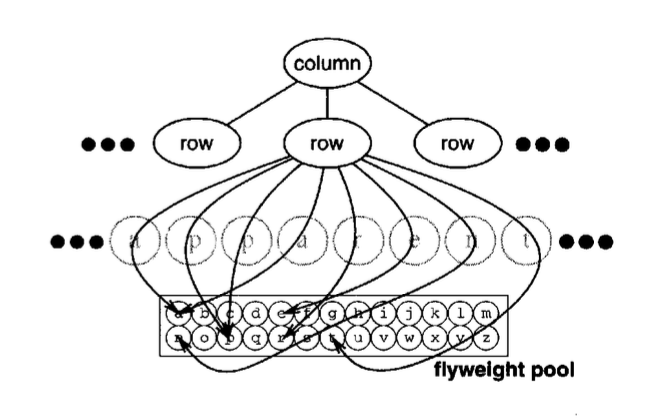
\includegraphics[width=1\linewidth]{assets/pattern/flyweight/flyweight-soluzione-2.png}
\end{figure}
\end{multicols}

\paragraph{Struttura} Il pattern è composto da:
\begin{itemize}
    \item \textbf{Flyweight}: dichiara un’interfaccia attraverso la quale gli oggetti flyweight possono ricevere lo stato esterno e agire di conseguenza.
    \item \textbf{FlyweightFactory}: crea e gestisce gli oggetti flyweight. Si assicura che i flyweight siano condivisi in modo appropriato. Quando un client richiede un flyweight, l’oggetto FlyweightFactory restituisce un’istanza esistente, oppure, se non esiste alcuna istanza, prima la crea e poi la restituisce.
    \item \textbf{Context}: contiene lo stato estrinseco, unico tra tutti gli oggetti originali. Quando un oggetto context è accoppiato con uno degli oggetti flyweight, rappresenta l’intero stato di un oggetto originale.
    \item \textbf{Client}: calcola oppure memorizza lo stato estrinseco dei flyweight. Dal punto di vista del client, un flyweight è un oggetto template che può essere configurato a tempo di esecuzione fornendogli dati contestuali come parametri dei suoi metodi.
\end{itemize}

\begin{figure}[H]
    \centering
    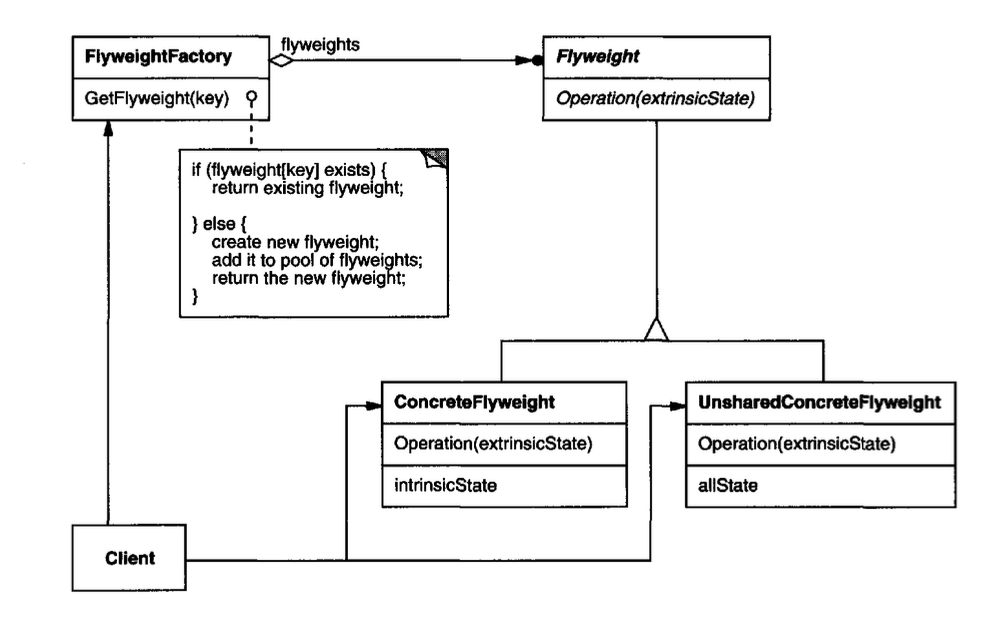
\includegraphics[width=0.75\linewidth]{assets/pattern/flyweight/flyweight-struttura.png}
    \caption{Class Diagram del pattern Flyweight}
\end{figure}

Lo stato intrinseco viene salvato nell'oggetto ConcreteFlyweight, mentre lo stato estrinseco è memorizzato o computato dal Client.

\begin{figure}[H]
    \centering
    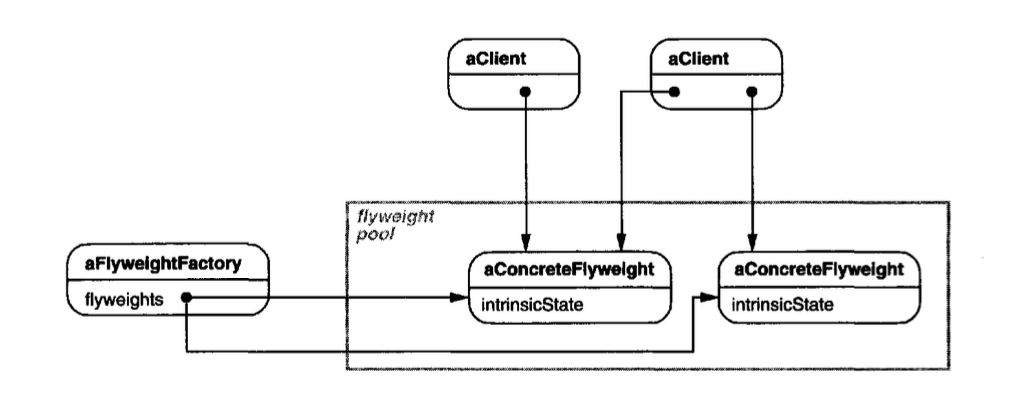
\includegraphics[width=0.75\linewidth]{assets/pattern/flyweight/flyweight-object-diagram.png}
    \caption{Object Diagram del pattern Flyweight}
\end{figure}

\paragraph{Conseguenze} Il pattern Flyweight consente quindi di:
\begin{itemize}
    \item Ridurre il numero totale di istanze condivise;
    \item Ammorbidire il costo spaziale dato dallo stato intrinseco;
\end{itemize}
È possibile affermare che maggiore è il numero di Flyweight condivisi, maggiore è lo spazio totale recuperato. Sebbene diminuisca il costo dato dallo stato intrinseco, aumenta quello dello stato estrinseco (in termini computazionali).



\newpage